\section{Análise no Tempo Contínuo}

\begin{frame}{Comportamento Dinâmico do Sistema}
  \begin{figure}
    \centering
    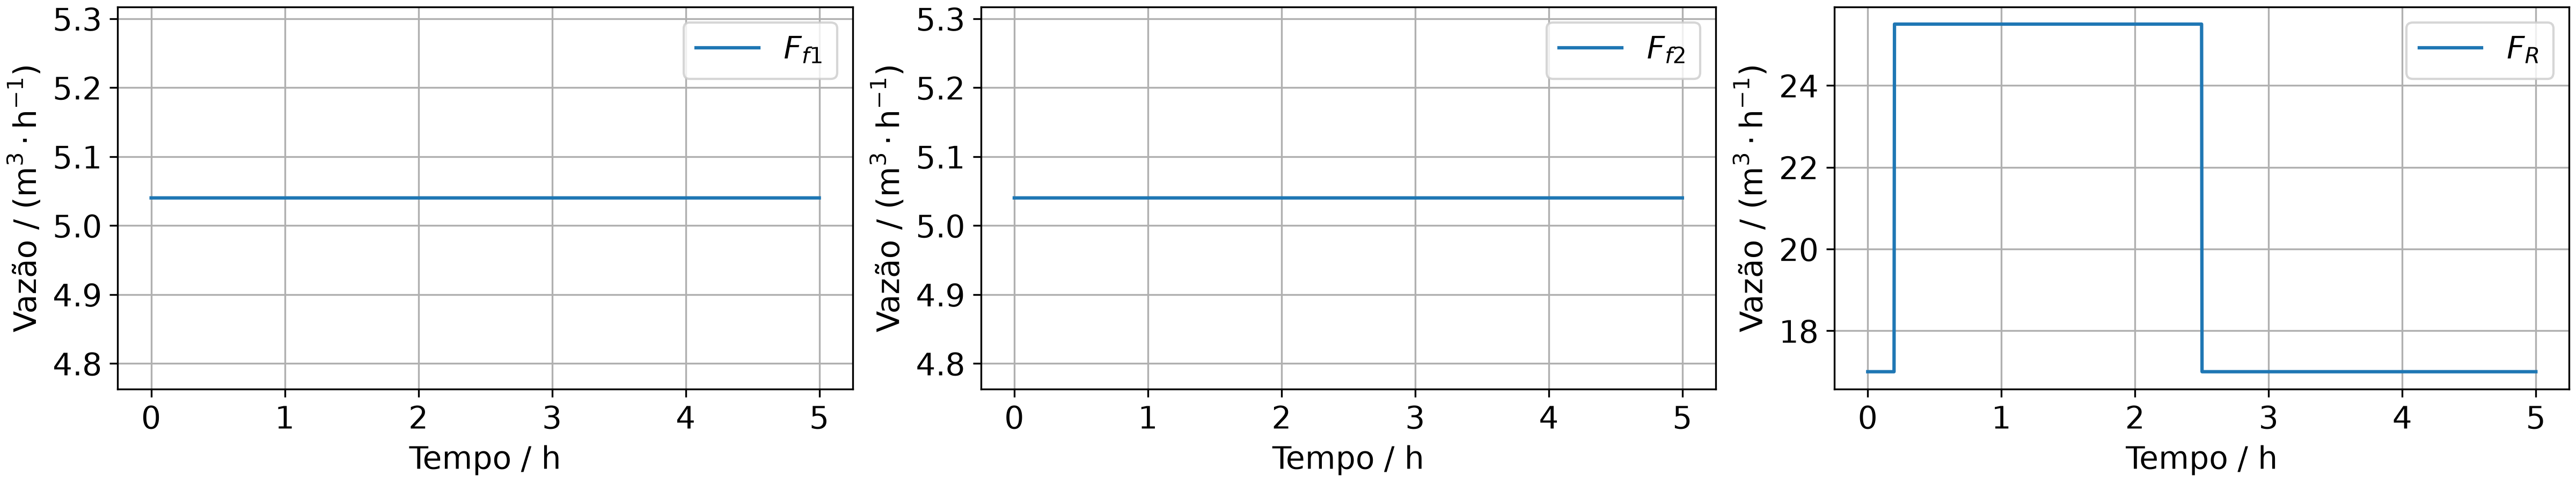
\includegraphics[width=0.8\linewidth]{../figures/nonlinear/pulse-FR-inputs.png}
    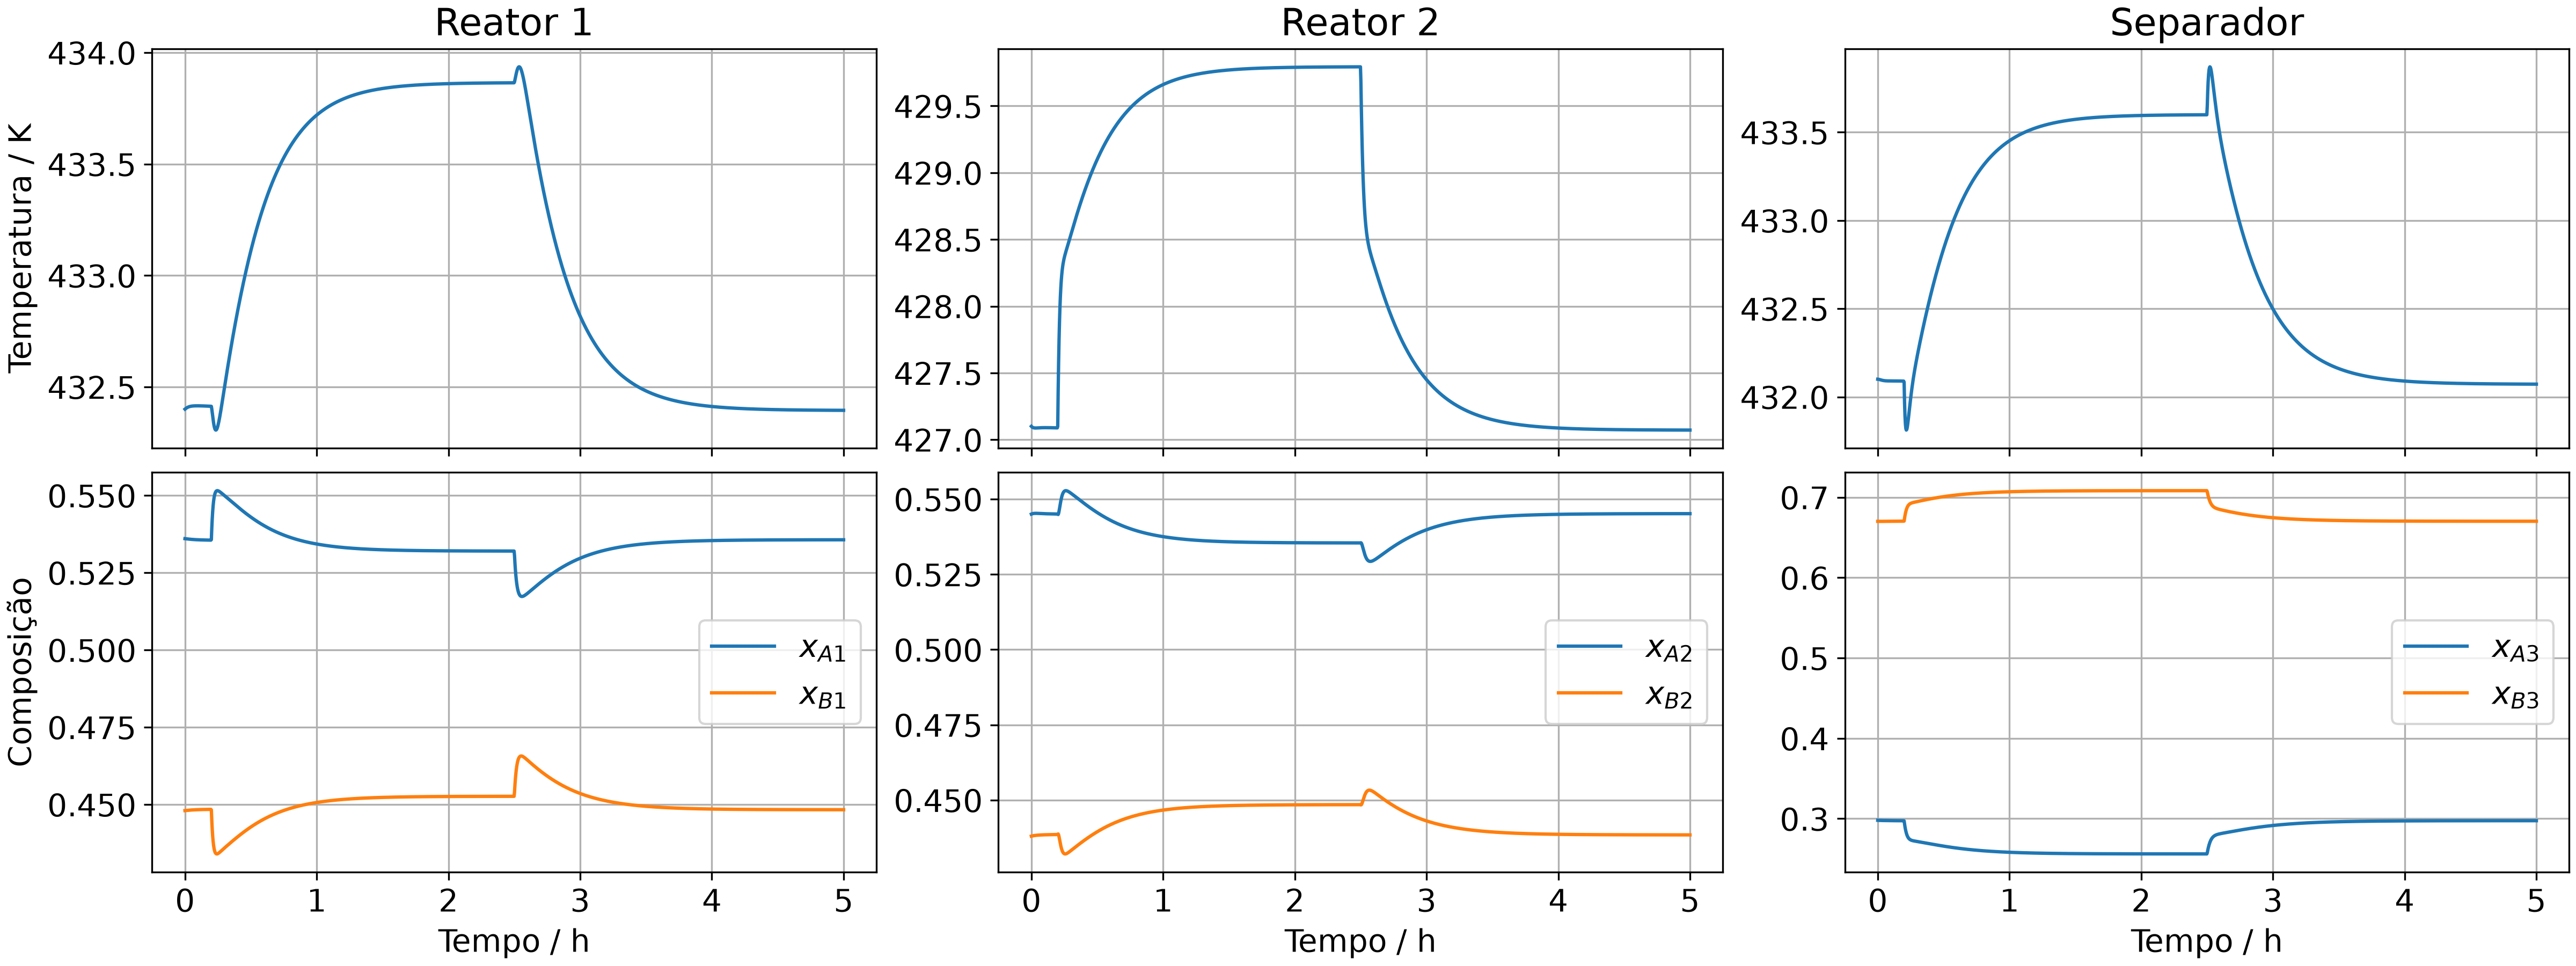
\includegraphics[width=0.8\linewidth]{../figures/nonlinear/pulse-FR-outputs.png}
    \caption{Entradas e saídas do sistema não linear para um pulso em $F_R$.}
  \end{figure}
\end{frame}

\begin{frame}{Linearização}
  O modelo foi linearizado em torno do ponto de operação de
  \citeonline{pourkargar_2017}:
  \vspace{-0.5cm}
  \begin{columns}[T]
    \column{0.5\textwidth}
    \begin{table}[h]
  \caption{Valores das variáveis de entrada no ponto de operação em regime estacionário ($u_{ss}$).}
  \label{tab:u_ss}
  \centering
  \begin{tabular}{lll}
    \hline
    Variável & Valor   & Unidade \\
    \hline
    $F_{f1}$ & 5{,}04  & m³/h    \\
    $F_{f2}$ & 5{,}04  & m³/h    \\
    $F_R$    & 17{,}00 & m³/h    \\
    \hline
  \end{tabular}
\end{table}

    \column{0.5\textwidth}
    \begin{table}[h]
  \caption{Valores dos estados do sistema no ponto de operação em regime estacionário ($y_{ss}$).}
  \label{tab:y_ss}
  \centering
  \begin{tabular}{lll}
    \hline
    Variável & Valor   & Unidade \\
    \hline
    $T_1$    & 432{,}4 & K       \\
    $T_2$    & 427{,}1 & K       \\
    $T_3$    & 432{,}1 & K       \\
    $x_{A1}$ & 0{,}536 & --      \\
    $x_{B1}$ & 0{,}448 & --      \\
    $x_{A2}$ & 0{,}545 & --      \\
    $x_{B2}$ & 0{,}438 & --      \\
    $x_{A3}$ & 0{,}298 & --      \\
    $x_{B3}$ & 0{,}670 & --      \\
    \hline
  \end{tabular}
\end{table}

  \end{columns}
\end{frame}

\begin{frame}{Comparação entre o modelo linear e não linear}
  \begin{columns}
    \column{0.5\textwidth}
    \begin{figure}
      \centering
      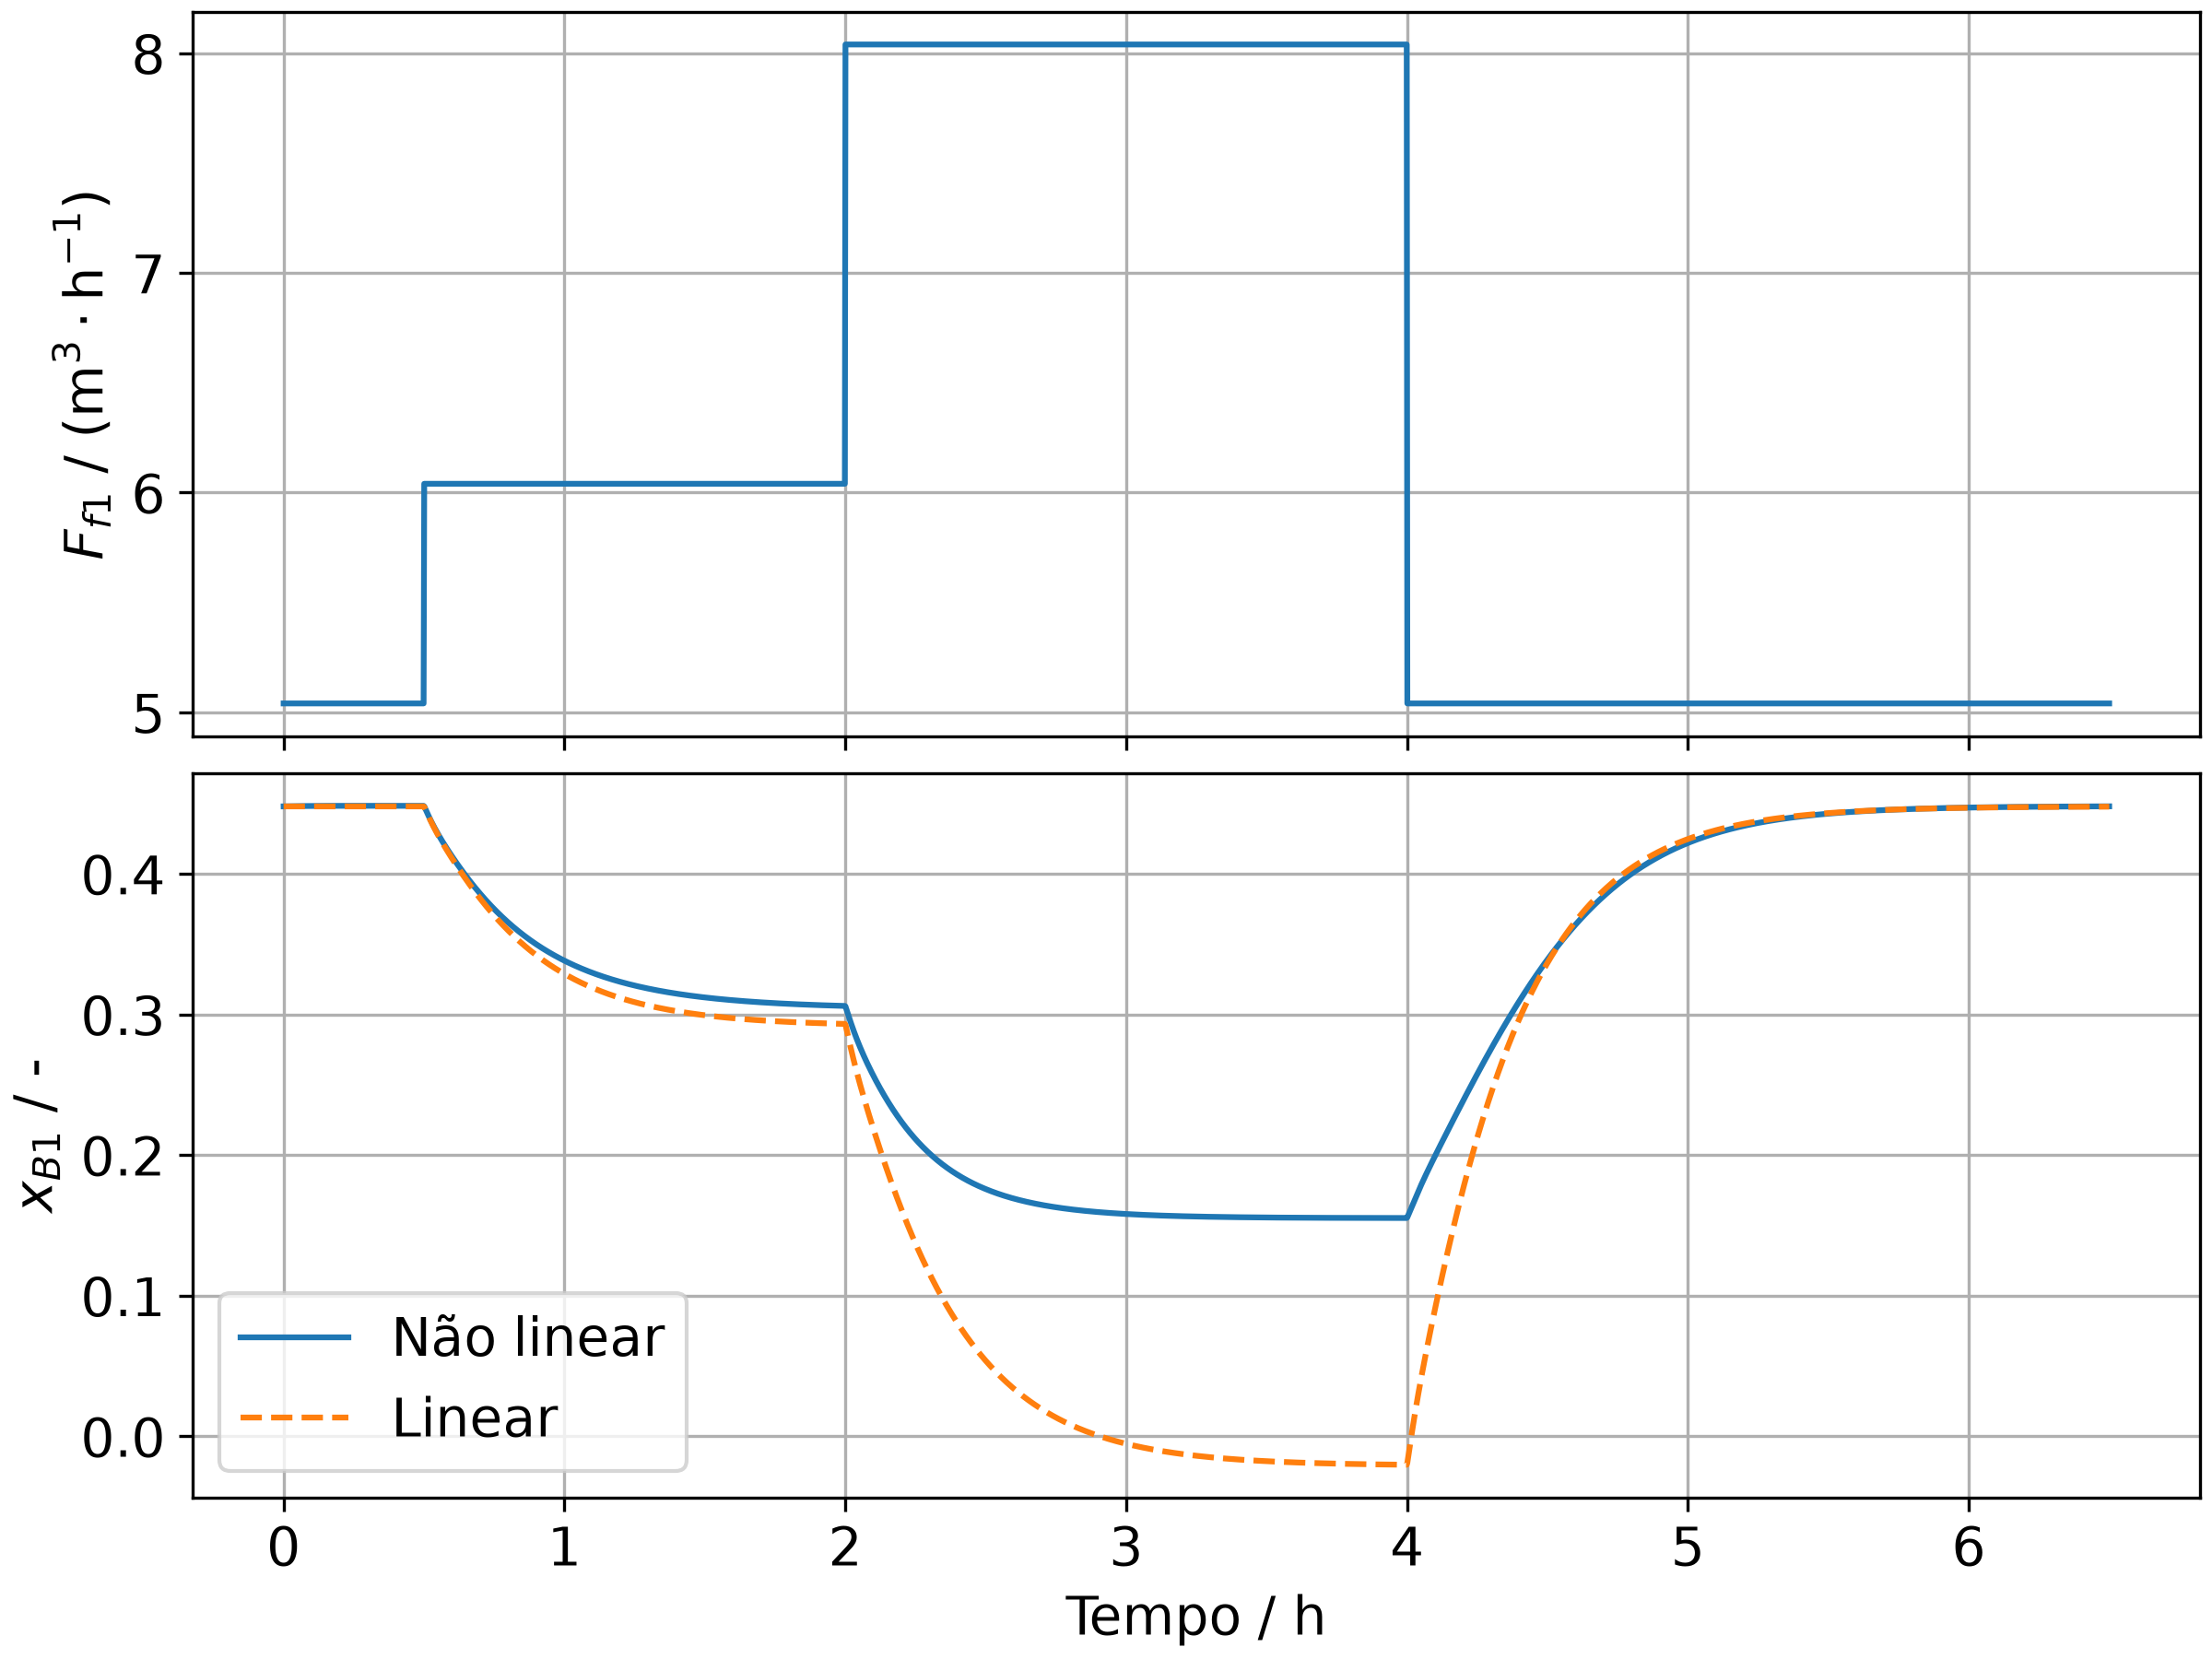
\includegraphics[width=\textwidth]{../figures/linear_vs_nonlinear/xB1_Ff1.png}
      \caption{Resposta da variável $x_{B1}$ a perturbações na entrada $F_{f1}$.}
    \end{figure}
    \column{0.5\textwidth}
    \begin{itemize}
      \item Boa concordância próxima ao ponto de linearização.
      \item As respostas divergem à medida que o sistema se afasta desse ponto.
      \item E o modelo linear prevê $x_{B1}<0$, sem significado físico, mostrando que a linearização é válida apenas localmente.
    \end{itemize}
  \end{columns}
\end{frame}
